
% ====================================
% chapter 2
% ====================================
\chapter{BinaryConnectによる良否判定}

% ******************************************************
% NeuralNetwork
% ******************************************************
\section{Neural Network}
Neural Networkとはニューロンと呼ばれる人間の脳細胞をもとに作られた数理モデルである.入力に対し重みをかけた時の出力から入力の特徴を抽出し分類問題を解く機械学習の1種である.


\subsection{Neural Networkの構造}
Neural Networkはユニットと呼ばれる最小要素を持ち,それに対し複数の入力と重み,バイアスから計算結果を出力する.
これらは図\ref{fig_NN1}のような構造をしており,入力$x_i$に対し重み$w_i$を乗算したものにバイアス$b$を足すことで出力$y$を得る.計算式は以下のように表される.
\begin{align}
y &= w_{1}x_{1} + w_{2}x_{2} + w_{3}x_{3} + b
\end{align}
\begin{figure}[htbp]
  \begin{center}
    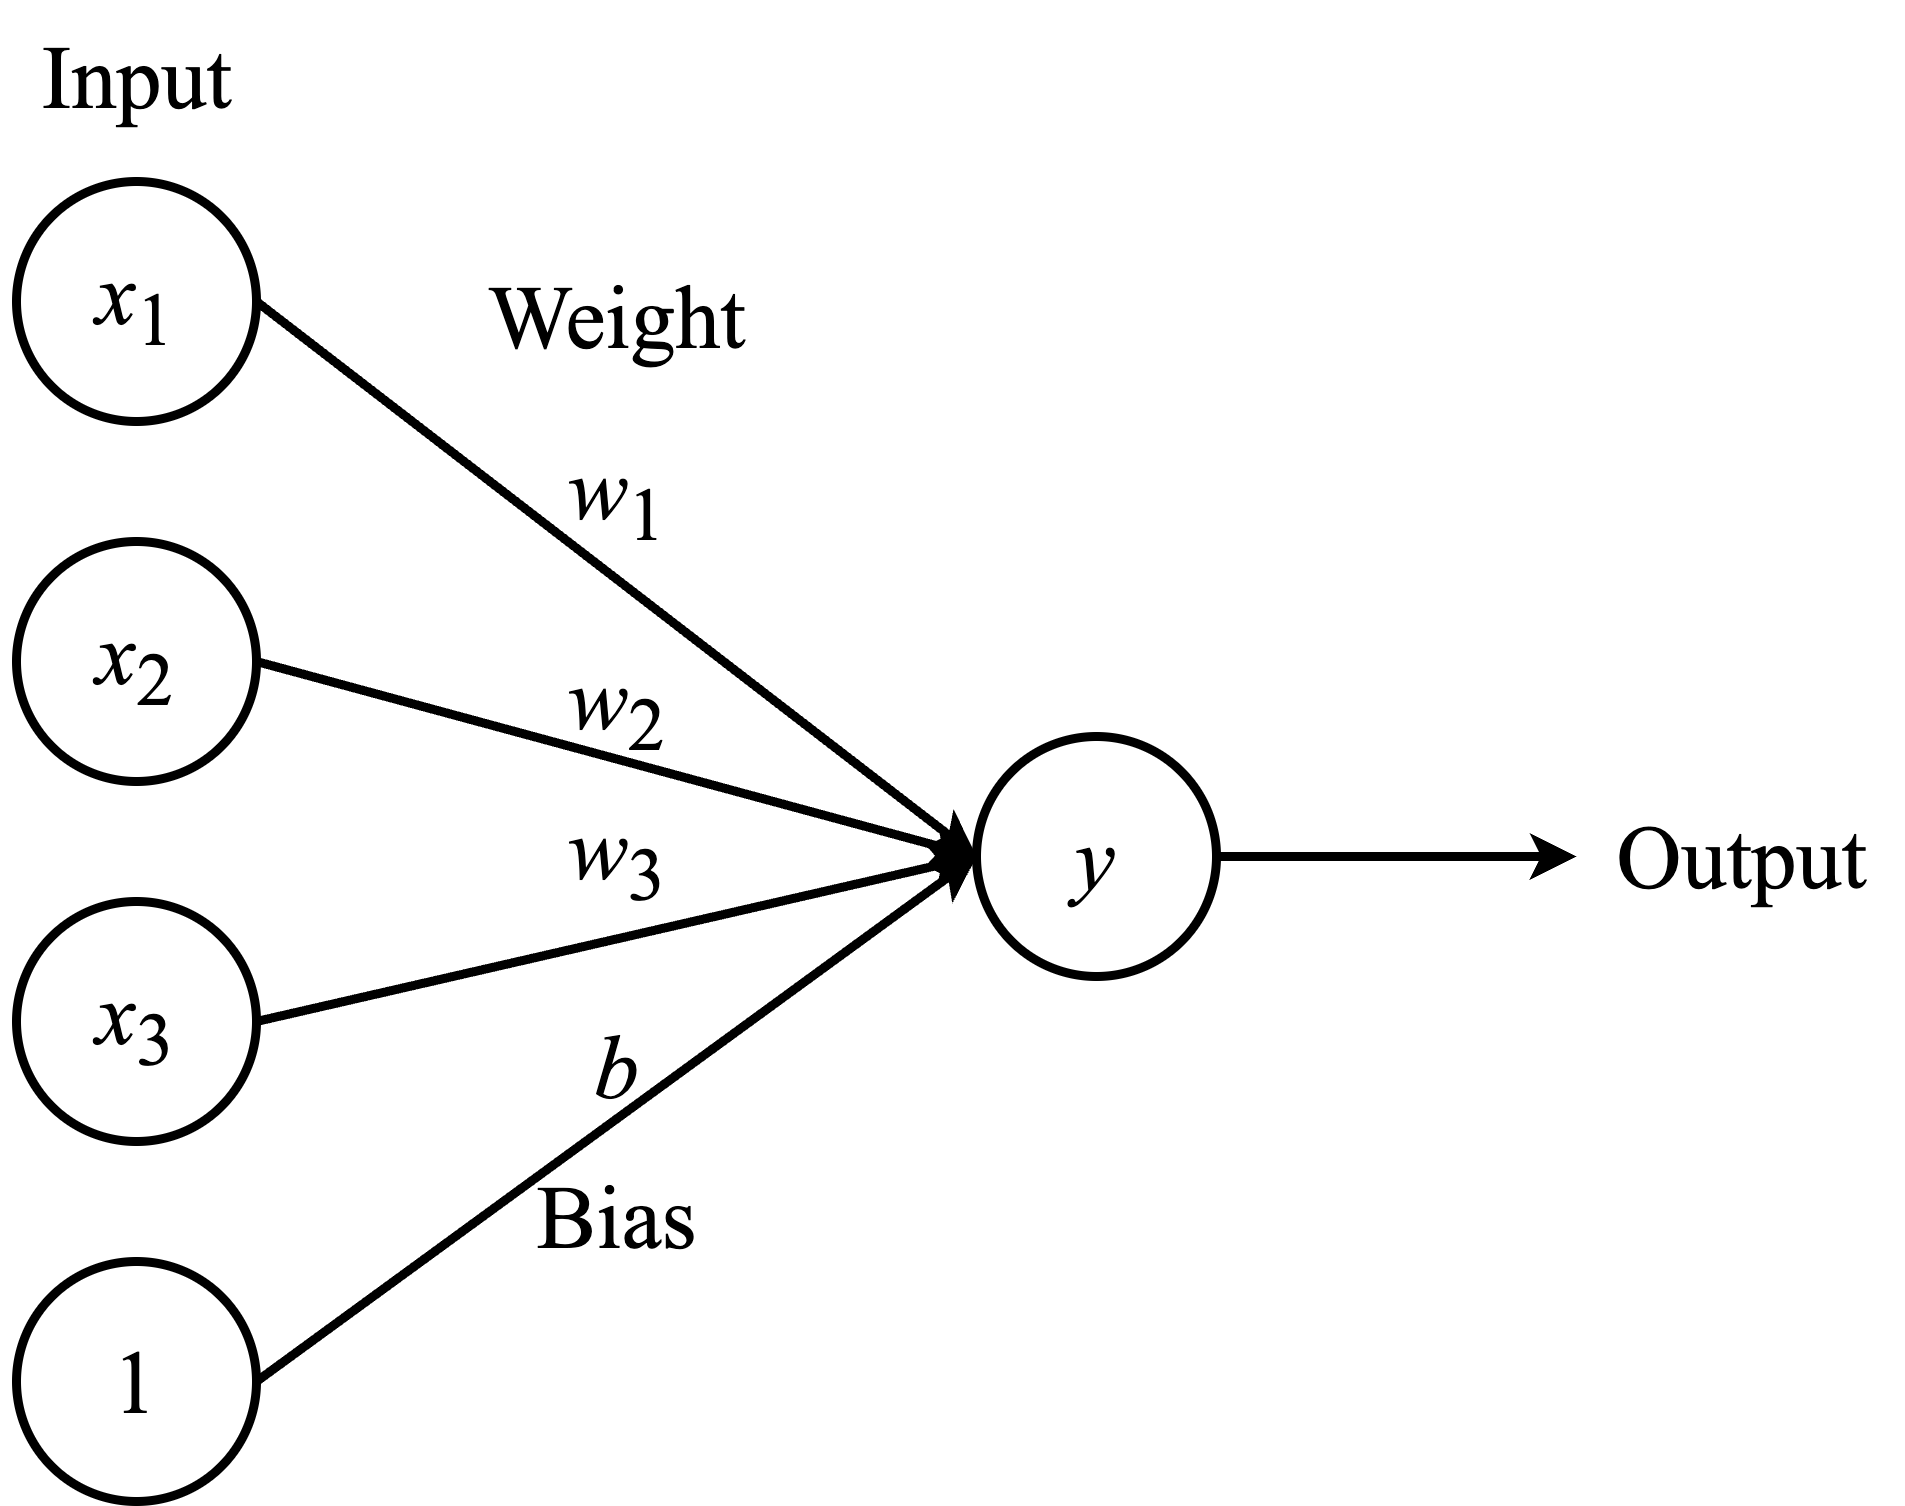
\includegraphics[scale = 0.13]{./chapter2/nn_1.png}
    \caption{ユニットの構造}
    \label{fig_NN1}
  \end{center}
\end{figure}

ここで出力$y$を複数個にすると,図\ref{fig_NN}のような構造になる.ユニットの縦方向の集まりのことを層と呼び,Neural Networkはこの層を複数組み合わせ,入力層・隠れ層・出力層という層を形成し計算を行う.
入力層$x$のユニットの個数を$i=1,2,3\ldots I$,隠れ層$z$のユニットの個数を$j=1,2,3\ldots J$とすると,それぞれの重みは$w_{j,i}$,バイアスは$b_j$となるため一般化した計算式は以下のようになる.
\begin{figure}[htbp]
  \begin{center}
    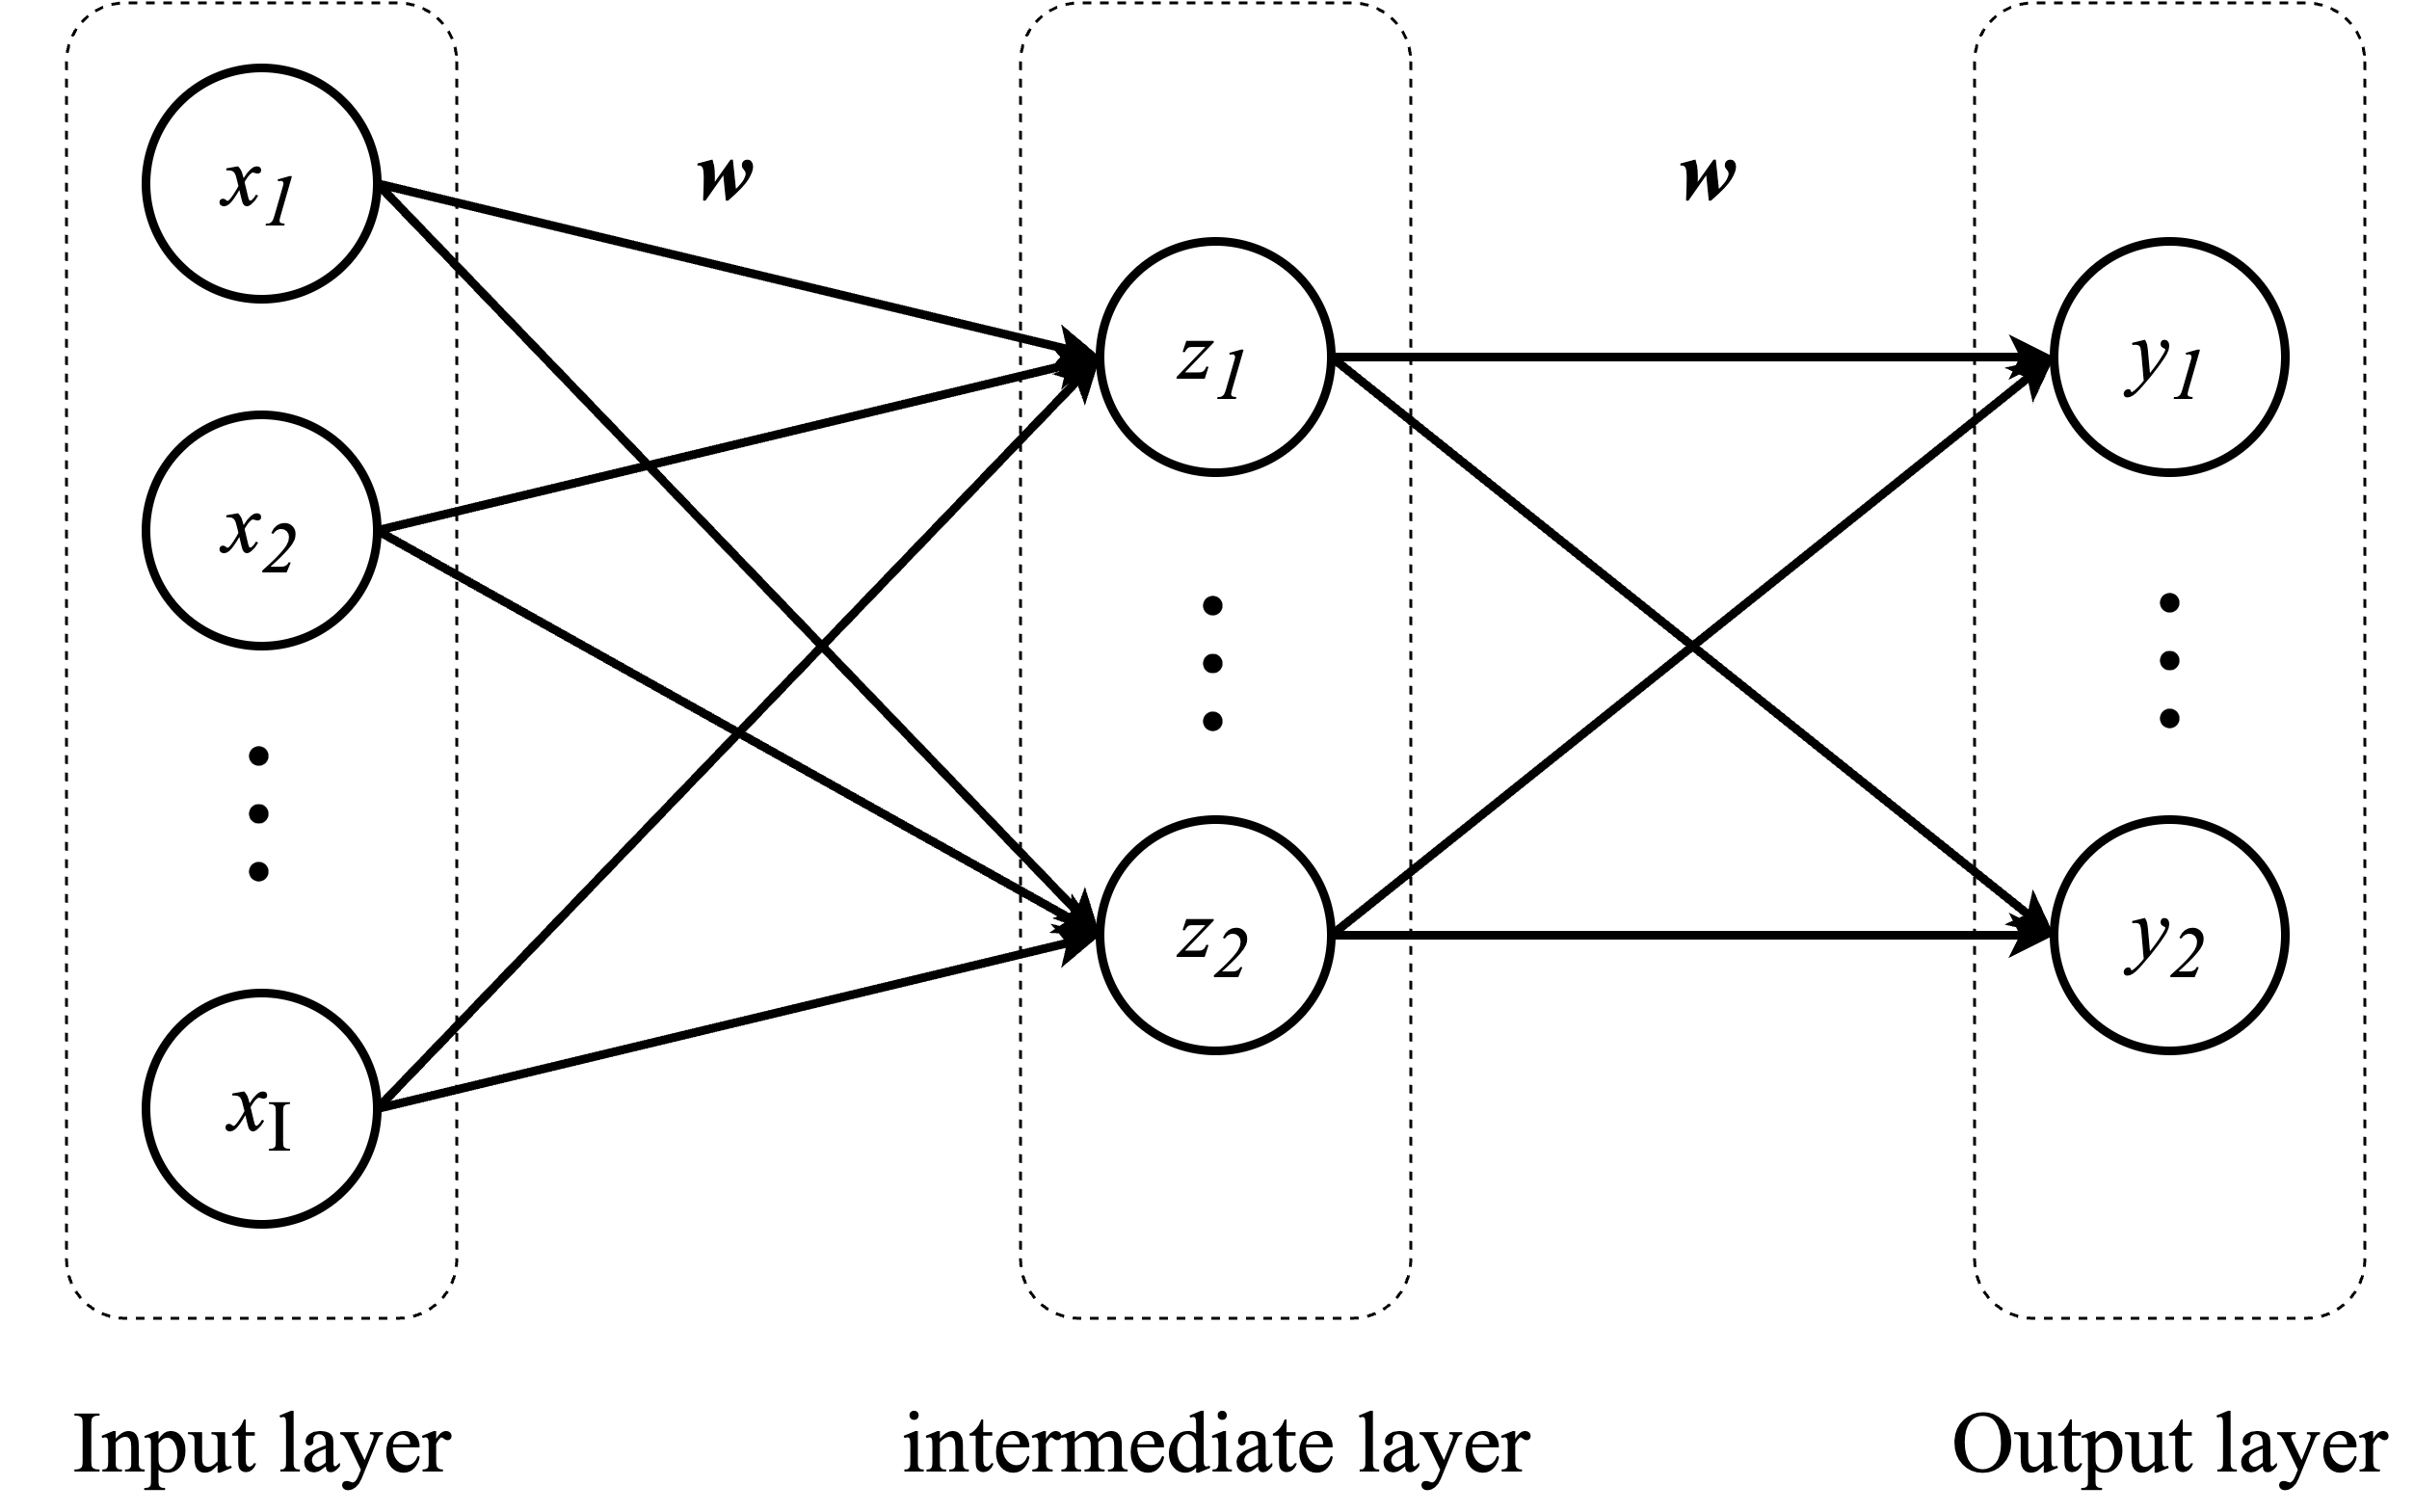
\includegraphics[scale = 0.13]{./chapter2/neural_network.png}
    \caption{Neural Networkの構造}
    \label{fig_NN}
  \end{center}
\end{figure}

\begin{align}
z_{j} &= \sum^{I}_{i=1}w_{j,i}x_{i} + b_j
\end{align}

ここで,各要素をベクトルと行列を用いて表し,次の層のユニットへの出力を一般化すると以下のような式となる.
\begin{align}
\bm{z} = \bm{W}\bm{x} + \bm{b}
\end{align}

隠れ層は1層のみである必要はなく,隠れ層の出力を次の層への入力として扱うことで層を多数化し,入力層から出力層までに多数の隠れ層を追加する.層数$L$のネットワークが存在する時,$l+1$層のユニットの出力$\bm{z}^{(l+1)}$は$l$層のユニットの出力$\bm{z}^{(l)}$から計算されるため,
\begin{align}
\bm{z}^{(l+1)} = \bm{W}^{(l+1)}\bm{z}^{(l)} + \bm{b}^{(l+1)}
\label{jundenpan}
\end{align}
という式で一般化される.したがって$l=1,2,3\ldots L-1$までの計算を順に行なっていくことで各層の出力を得ることができ,最終的な出力$\bm{y}=\bm{z}^{(L)}$を計算することができる.このような構造の層を全結合層と呼ぶことが多い.


\subsection{学習による重みの更新}
前項のような計算により,入力が与えられたときの出力を得ることができ,このときの出力がNeural Networkが導いた推論になる.教師あり学習の場合,入力に対し求められる出力が正解として与えられる.その正解と,入力からネットワークによって求められた推論を比較し,より求められる正解に推論が近づくように重みを更新していくのである.

例えば0から9までの手書き文字が入力として与えられその分類を行うとき,出力は$y_0, y_1, \ldots , y_9$までの10個の出力を用意する.10個の出力に対し0から9までの数字を対応させ出力が1になった数字を推論として扱う.その時の構造を図\ref{fig_study}に示す.
\begin{figure}[htbp]
  \begin{center}
    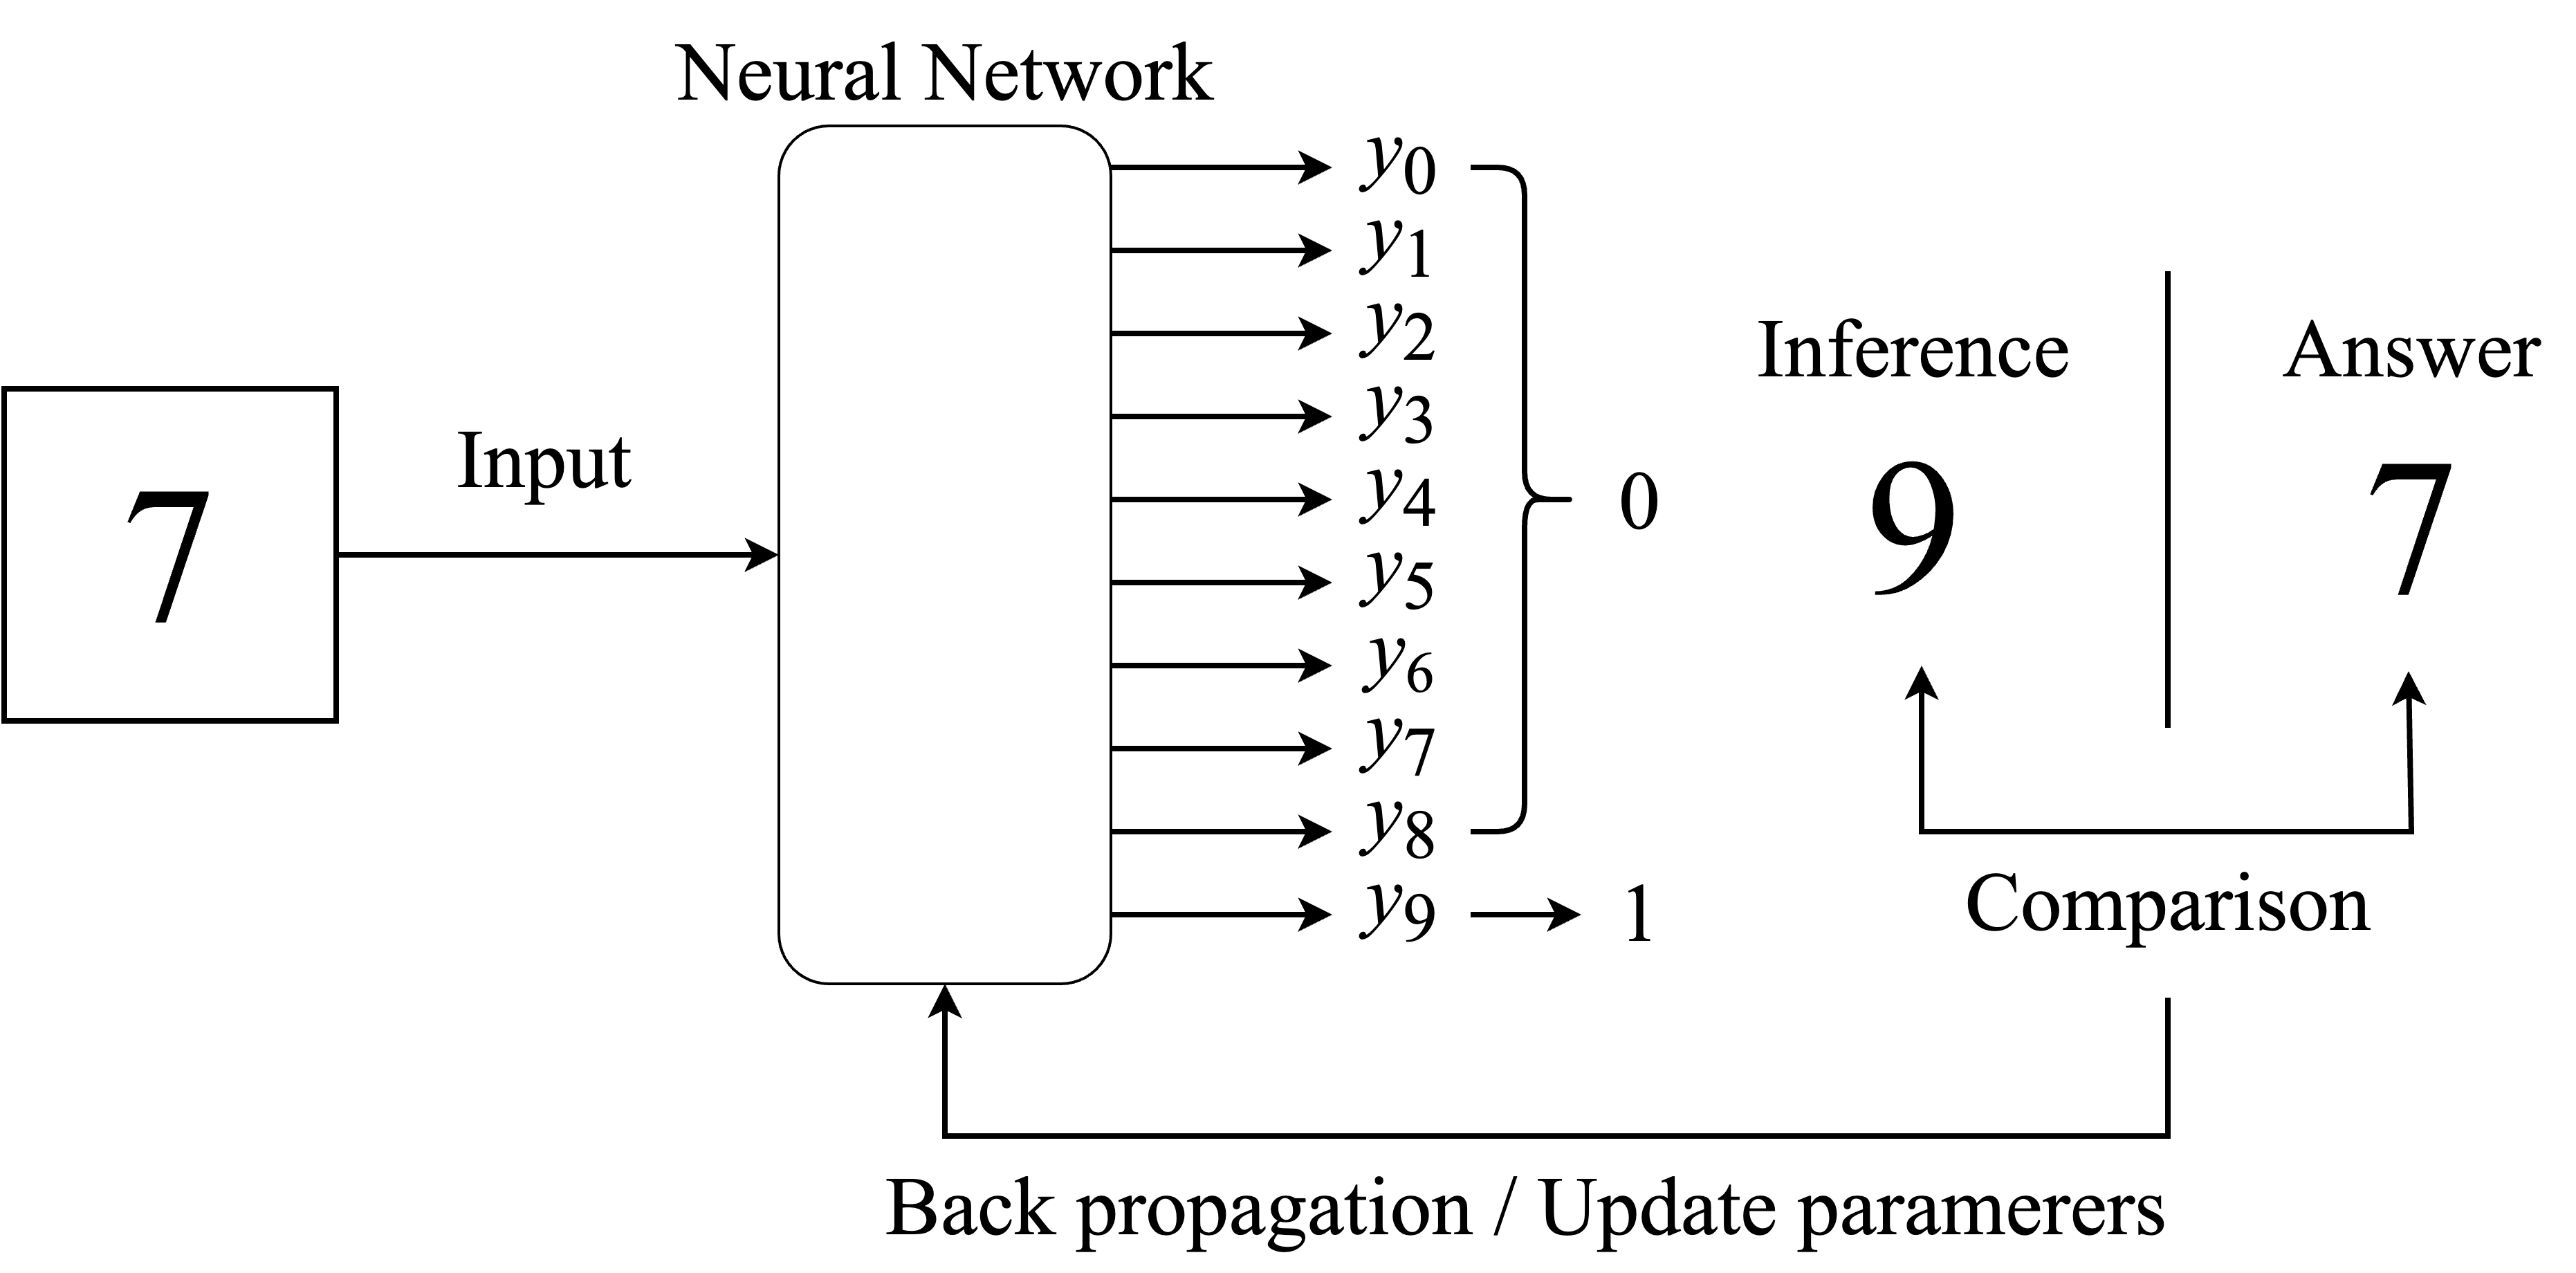
\includegraphics[scale = 0.1]{./chapter2/NN_study.png}
    \caption{Neural Networkにおける学習の流れ}
    \label{fig_study}
  \end{center}
\end{figure}

このとき,実際の答えは7だが推論の結果は9となり不正解になる.そこで両者を比較し誤差逆伝播を行うことでNeural Network内のパラメータをどのように変更すれば推論を正解に近づけることができるかを求める.そして重みを更新していき推論が正解に近づいていくように変更していくのがNeural Networkにおける機械学習である\cite{sinsou}.

\subsection{誤差逆伝播}
前項で述べたようなNeural Networkのパラメータの更新には勾配降下法が用いられる.これは損失関数を微分し,勾配のベクトルを求めることで重みを更新していく手法である.しかし,Neural Networkではある層での出力が次の層への入力へとつながっているため,入力に近い層のパラメータであるほど微分計算の中に次の層のパラメータが現れ,微分の連鎖則を何度も繰り返すことになる.

そこで,この勾配計算を効率よく行うための手法が誤差逆伝播である.式\ref{jundenpan}による計算で順伝播を行った際,出力層では出力$\bm{z}^{(L)}$と誤差$\bm{d}^{(L)}$を得る.ここで,誤差関数を層の入力によって微分したものをデルタとすると,出力層のデルタ$\delta^{(L)}$は以下のようになる.
\begin{align}
  \bm{\delta}^{(L)} = \bm{z}^{(L)} - \bm{d}^{(L)}
\end{align}

この結果を元に,中間層$l = L-1,L-2,L-3,\ldots 2$での各ユニット$j$でのデルタ$\delta^{(l)}_j$を以下の式によって計算する.
\begin{align}
  \delta^{(l)}_j = \sum_k \delta^{(l+1)}_k (w^{(l+1)}_{kj} f'(u^{(l)}_k))
\end{align}

求めた微分を元に各層のパラメータ$w^{(l)}_{ji}$に関する微分を以下式によって計算する.
\begin{align}
  \frac{\partial \bm{E}_n}{\partial w^{(l)}_{ji}} = \delta^{(l)}_j z^{(l-1)_j}
  \label{gyakudennpann}
\end{align}

これによって,本来全層にわたって微分する必要のあった勾配計算を効率よく求めることができる.また,\ref{gyakudennpann}は誤差関数をパラメータによって微分したものであるが,これは$w$を増加させた時に誤差が増加する量と捉えることができる.そのため,誤差を減少させる方向にパラメータを更新するには以下の式に従う.ここで,$\eta$は学習率であり,パラメータ更新の量を決定する.
\begin{align}
  \bm{w} \gets \bm{w} - \eta \frac{\partial \bm{E}_n}{\partial w^{(l)}_{ji}}
  \label{gyakudennpann}
\end{align}

% ******************************************************
% CNN
% ******************************************************
\section{CNN}
\subsection{学習の概要}
CNNとは畳み込みと呼ばれる画像処理を組み込んだNeural Networkの1種で,画像分類など画像を用いた学習を得意としている.Neural Networkに畳み込み層を追加したものがCNNであるが,畳み込み層における画像,フィルタがNeural Networkにおける入力,重みとなっている.
CNNでは主に畳み込みとプーリングという処理を用いて画像の特徴を抽出し学習を行っている.


\subsection{畳み込み}
畳み込みとは画像に対してフィルタをかけ,フィルタと類似する濃淡パターンを検出する役割を持つ.
畳み込み層を考える上で,図\ref{fig_conv}のように$I \times J$ピクセルの画像と$2 \times 2$の要素を持つフィルタが存在すると考える.
\begin{figure}[htbp]
  \begin{center}
    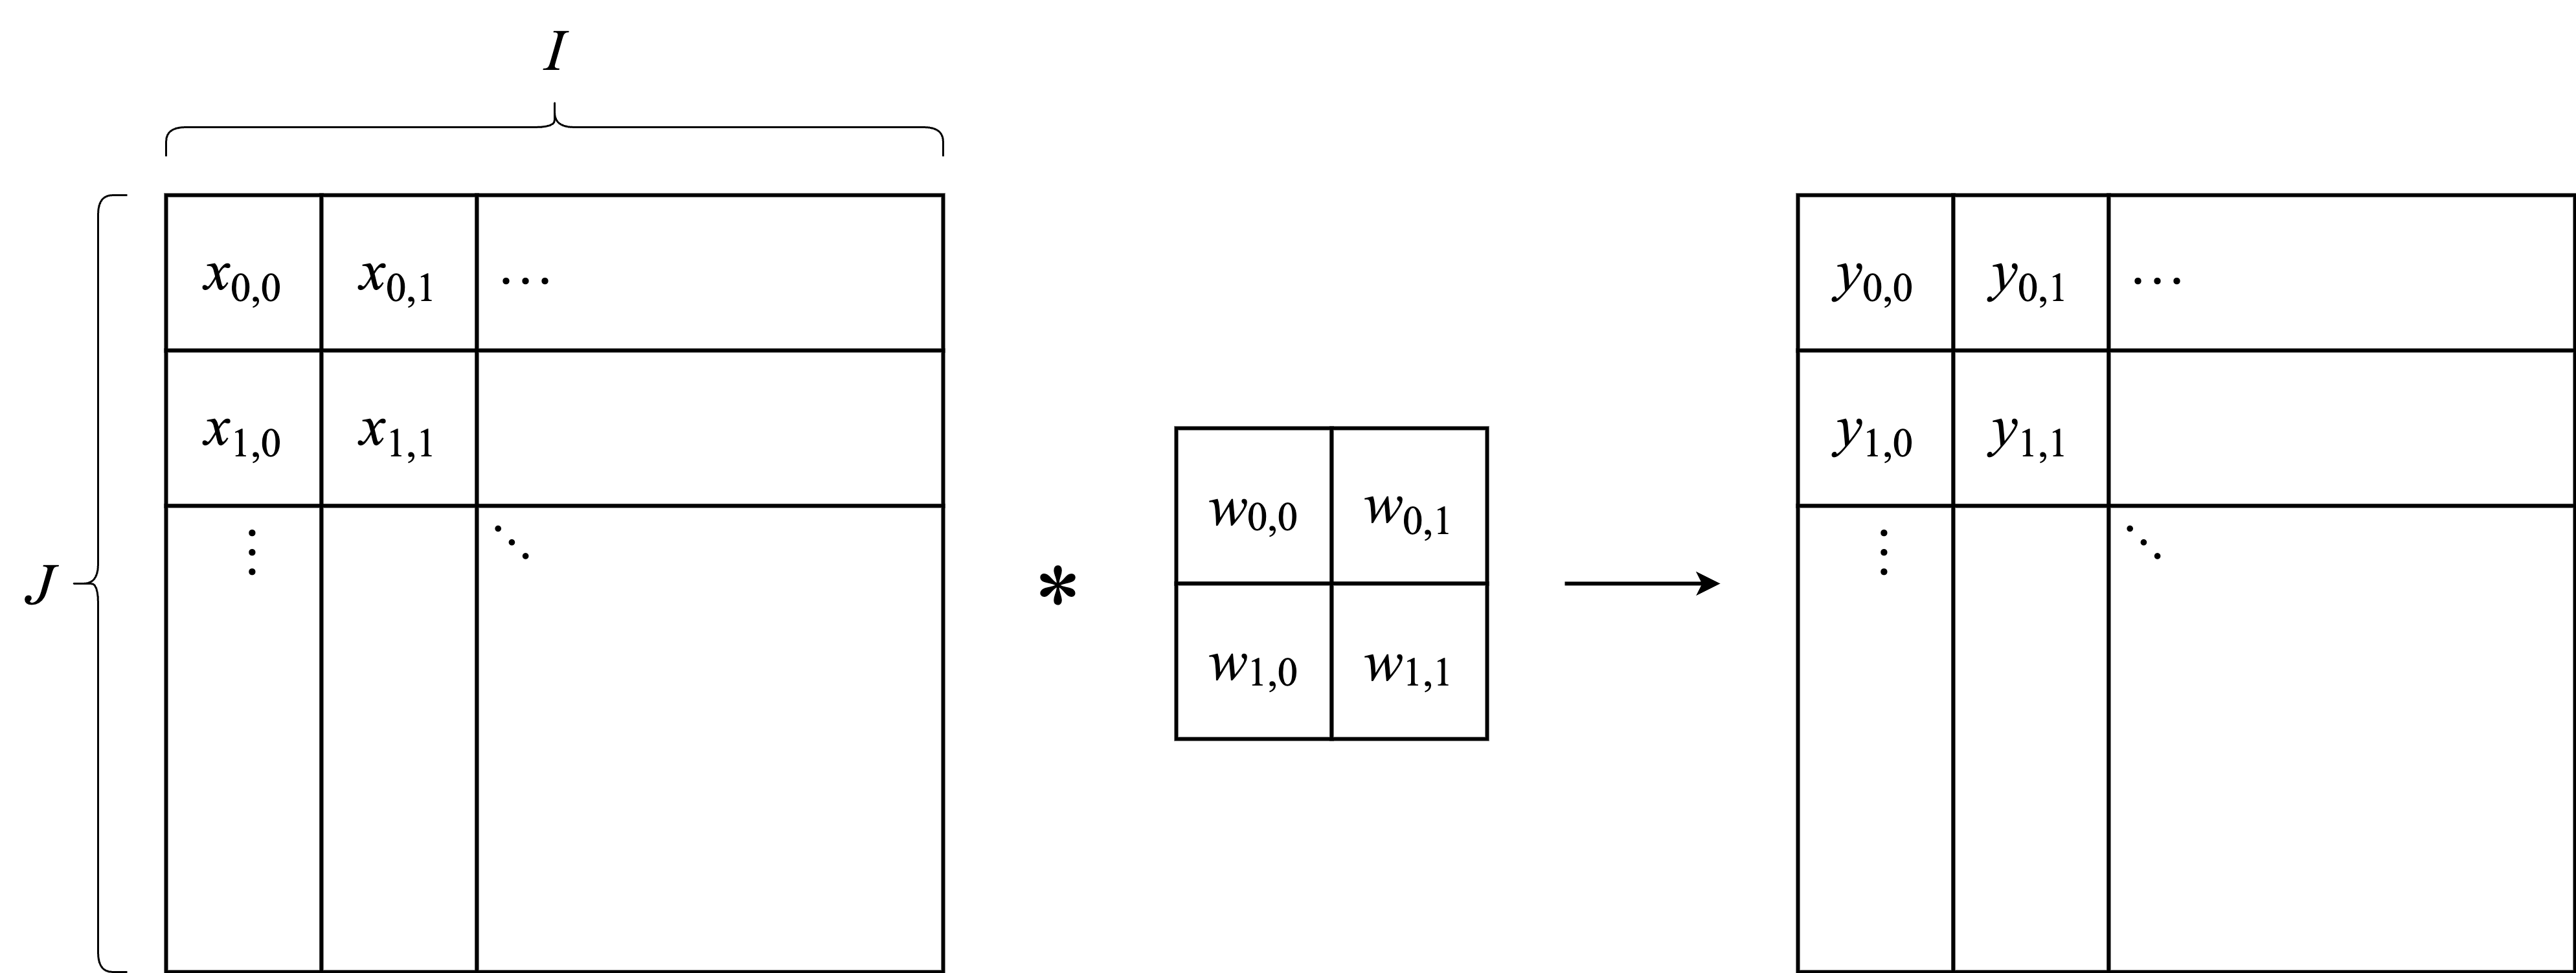
\includegraphics[scale = 0.1]{./chapter2/cnn_tatamikomi.png}
    \caption{畳み込みの計算}
    \label{fig_conv}
  \end{center}
\end{figure}

ここでフィルタを$x_{00}$に重ねるように置き,各要素について乗算したものの和を出力とすると以下のように計算できる.
\begin{align}
  y_{0,0} = x_{0,0}w_{0,0} + x_{0,1}w_{0,1} + x_{1,0}w_{1,0} + x_{1,1}w_{1,1}
  \label{fig_NN1}
\end{align}

畳み込み層ではフィルターを1ピクセルずつスライドさせながら同じ計算をする.出力$y$のインデックスを$i,j$とし,フィルタのサイズを$W\times H$,とすると出力は以下の式で一般化できる.
\begin{align}
  y_{i,j} = \sum^{W-1}_{p=0} \sum^{H-1}_{q=0} x_{i-p,j-q}w_{p,q}
\end{align}
CNNではこの計算を繰り返していくことで画像の特徴を抽出する.

このままでは入力の画像に対し出力画像が1ピクセル分小さくなってしまうため,前後で画像サイズを変更したくない場合はパディングと呼ばれる入力画像の外側に情報を追加する処理を行う.よく使用されているのは0パディングと呼ばれる画像の外側1ピクセル分を0で埋め尽くす処理である.

また,通常のNeural Networkと同様に入力には複数枚の画像を使用する.複数の画像に同一のフィルタを畳み込み,それを足し合わせることで出力を得る.フィルタは層ごとに増やしていき,フィルターの数だけ画像のch数は増えていく.これを図に表すと図\ref{fig_cnn_ch}のようになる.
\begin{figure}[htbp]
  \begin{center}
    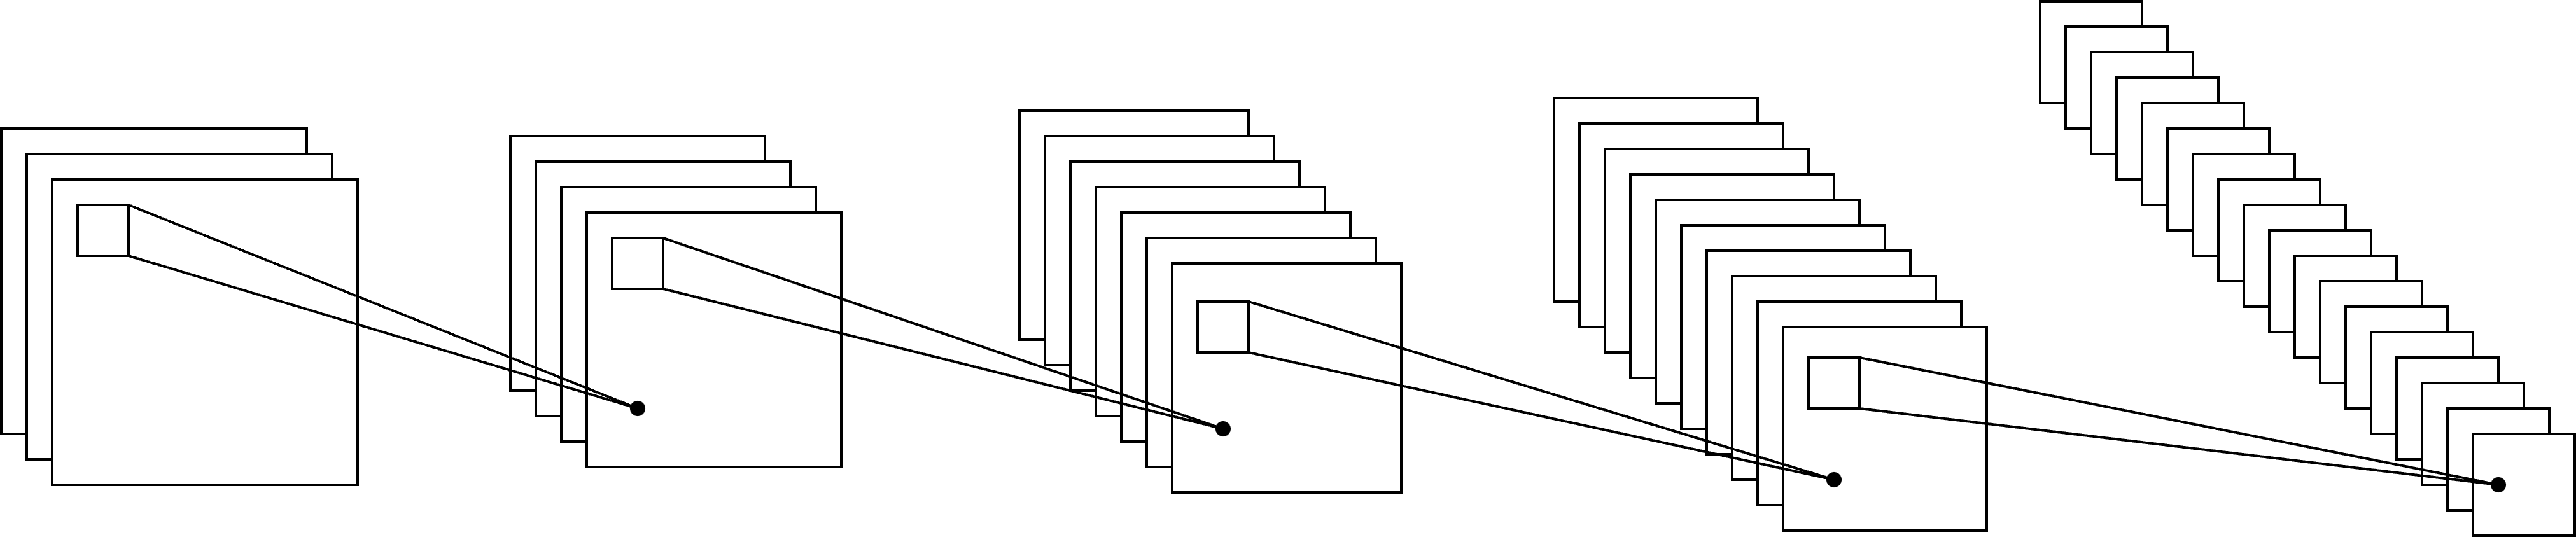
\includegraphics[scale = 0.05]{./chapter2/cnn_ch.png}
    \caption{畳み込み層での計算の概要}
    \label{fig_cnn_ch}
  \end{center}
\end{figure}

\subsection{プーリング}
プーリングとは畳み込みで取得した画像の特徴を増幅させるような処理である.畳み込みを行った画像に対し,あらかじめ指定したサイズで画像を分割しその分割ごとに情報を要約することと,解像度を落としダウンサンプリングさせるような2つの効果を持つ.この2つの処理によって入力信号の平滑化とダウンサンプリングによるエイリアシングの防止をになっている.

プーリングにはいくつかの種類が存在する.その中でも最も一般的な手法が図\ref{fig_pooling}に示すような最大値プーリングである.これは入力画像を指定したパディングサイズごとに分割して,その分割内の最大値を出力とする手法である\cite{sinsou}.
\begin{figure}[htbp]
  \begin{center}
    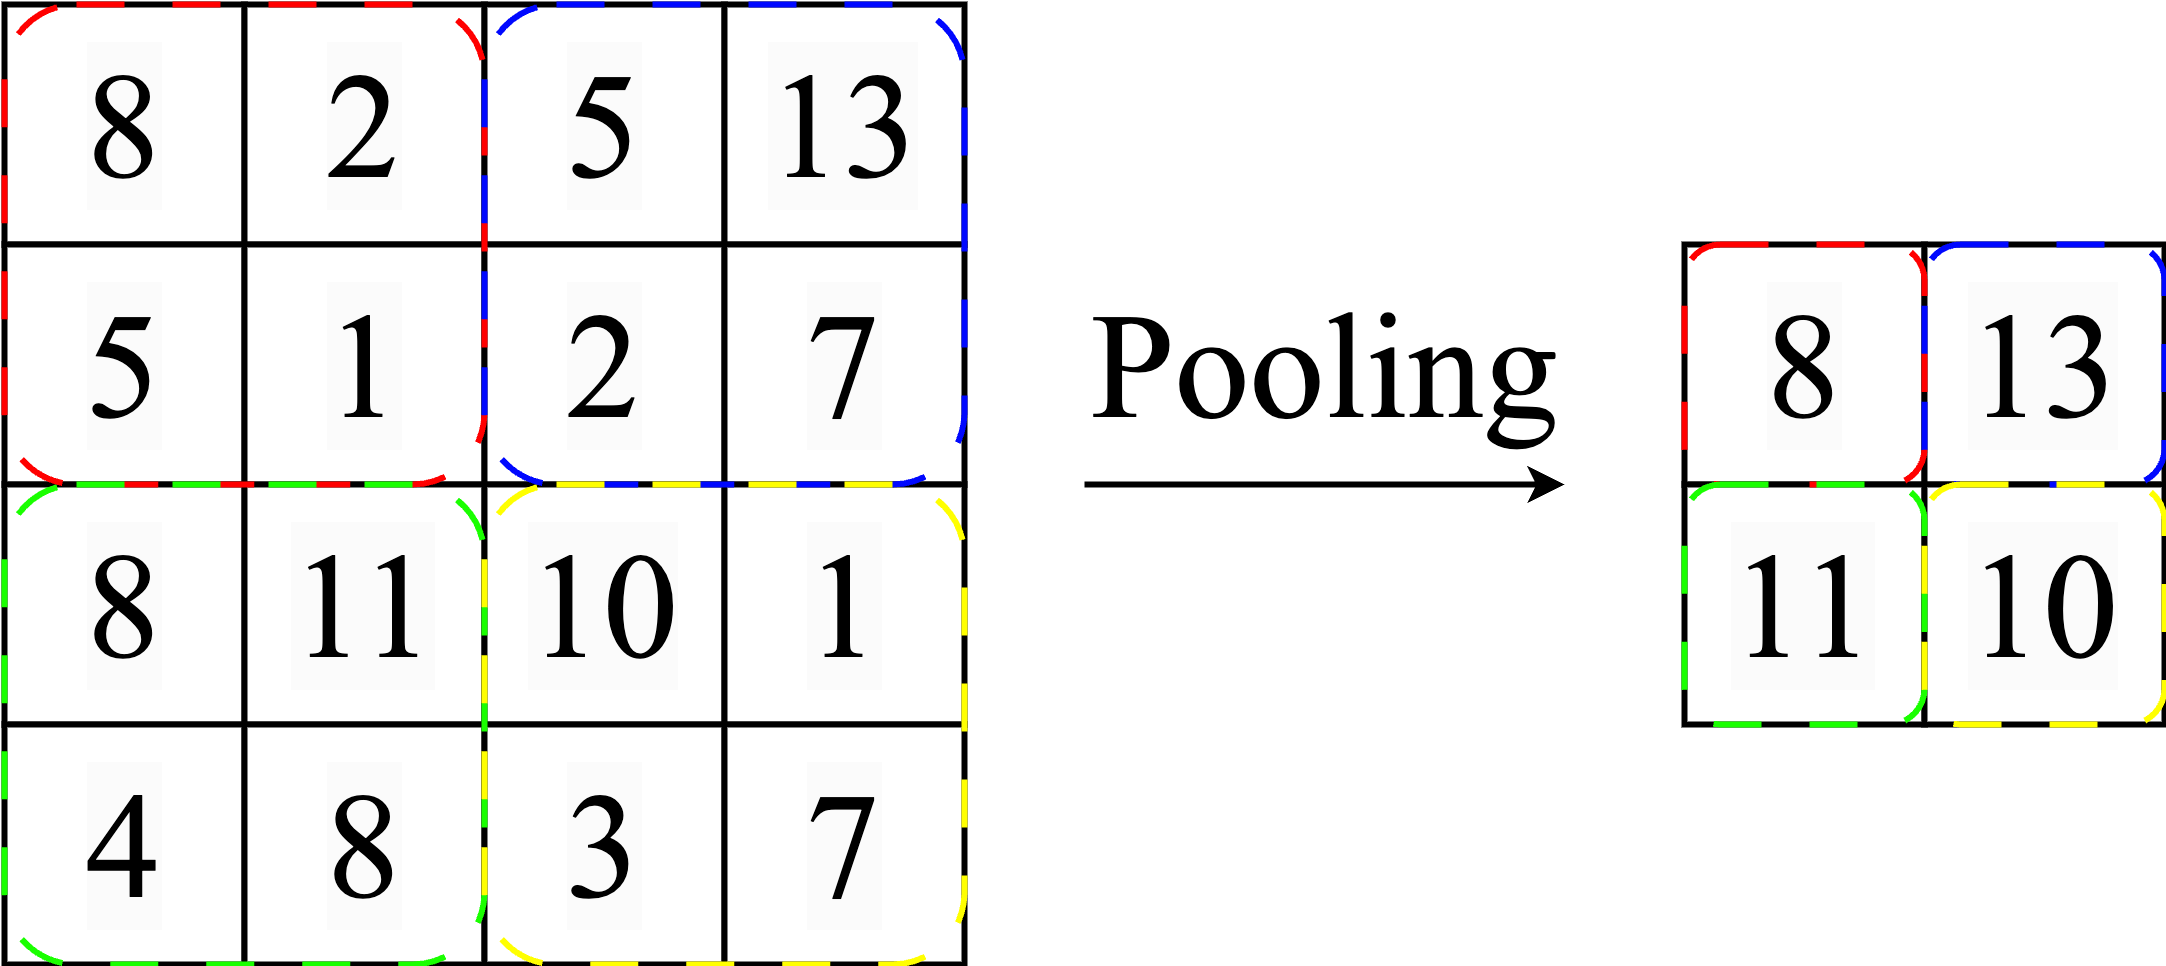
\includegraphics[scale = 0.13]{./chapter2/pooling.png}
    \caption{最大値プーリング}
    \label{fig_pooling}
  \end{center}
\end{figure}

\subsection{Batch Normalization}
Batch Normalizationhaとはミニバッチ内の全サンプルにわたるそのユニットの出力の平均と分散を求め正規化する手法である.畳み込み層ではチャンネル毎に入力に対し同一のフィルタを適用するため正規化に必要な平均と分散はチャンネルごとに求める.CNNではミニバッチ毎やレイヤー毎に特徴量の分布が違うことがあるが,この処理を行うことで各特徴量の平均をゼロに標準偏差を1にし,分布の偏りやスケールの影響を排除することができる.

ミニバッチ内のサンプルを$n=1,2,\ldots,3$とし,畳み込み層のチャンネル$c$を構成する$W\times H$内の位置$(i,j)$のユニットへの層入力を$u^{(n)_ijc}$と表した時,全ての$i,j,n$にわたる平均を以下のように求める.
\begin{align}
  \mu_c = \frac{1}{NWH} \sum_{i,j,n} u^{(n)}_{ijc}
\end{align}

同じ値の集合に対する分散$\sigma^2_c$とすると,$u^{(n)}_{ijc}$は以下の式で正規化される.ここで,$\gamma_c$と$\beta_c$は定数であり学習によって求めるパラメータである.
\begin{align}
  \hat{u}^{(n)}_{ijc} = \gamma_c \frac{u^{(n)}_{ijc} - \mu_c}{\sqrt{\sigma^2_c + \varepsilon}} + \beta_c
\end{align}


% ******************************************************
% BinaryConnect
% ******************************************************
\section{BinaryConnect}
BinaryConnectとはNeuralNetworkにおける重みを1と-1に2値化する手法である.浮動小数の重みを$\bm{w}$,2値化した重みを$\bm{w}_b$とすると,$\bm{w}_b$は以下のように計算される.
\begin{displaymath}
  \bm{w_{b}} = \left\{ \begin{array}{l}
  \displaystyle 
  +1\:  \text{if}\:  \bm{w} > 0 \\
  -1\:\text{otherwise}
  \end{array} \right.
\end{displaymath}

通常のNeural Networkの重みは32bitまたは16bitの浮動小数点で表されるが,BinaryConnectでは1,-1ネットワーク内で0,1に対応させ,1bitで表すことができる.これにより重みのメモリ使用量は32分の1まで抑えることが可能である.

また,前章より図\ref{fig_conv}での畳み込み層での計算は式\ref{fig_NN1}で計算されるが,重みを全て1,-1にすることによって以下の式のように入力と重みの乗算を加減算のみで表すことができるようになる.
\begin{align}
  y_{0,0} = x_{0,0} \pm x_{0,1} \pm x_{1,0} \pm x_{1,1}
\end{align}
これにより,ネットワーク中の乗算器を加算機に置き換えることができるため計算リソースの削減をすることができる

学習における勾配の蓄積や重みの更新は一般的なCNN通り,浮動小数の重みに対して処理し,推論時に使用する重みのみ2値化の処理をする.図\ref{fig_binarize} に処理の流れを示す\cite{courbariaux2016binaryconnect}.
\begin{figure}[htbp]
  \begin{center}
    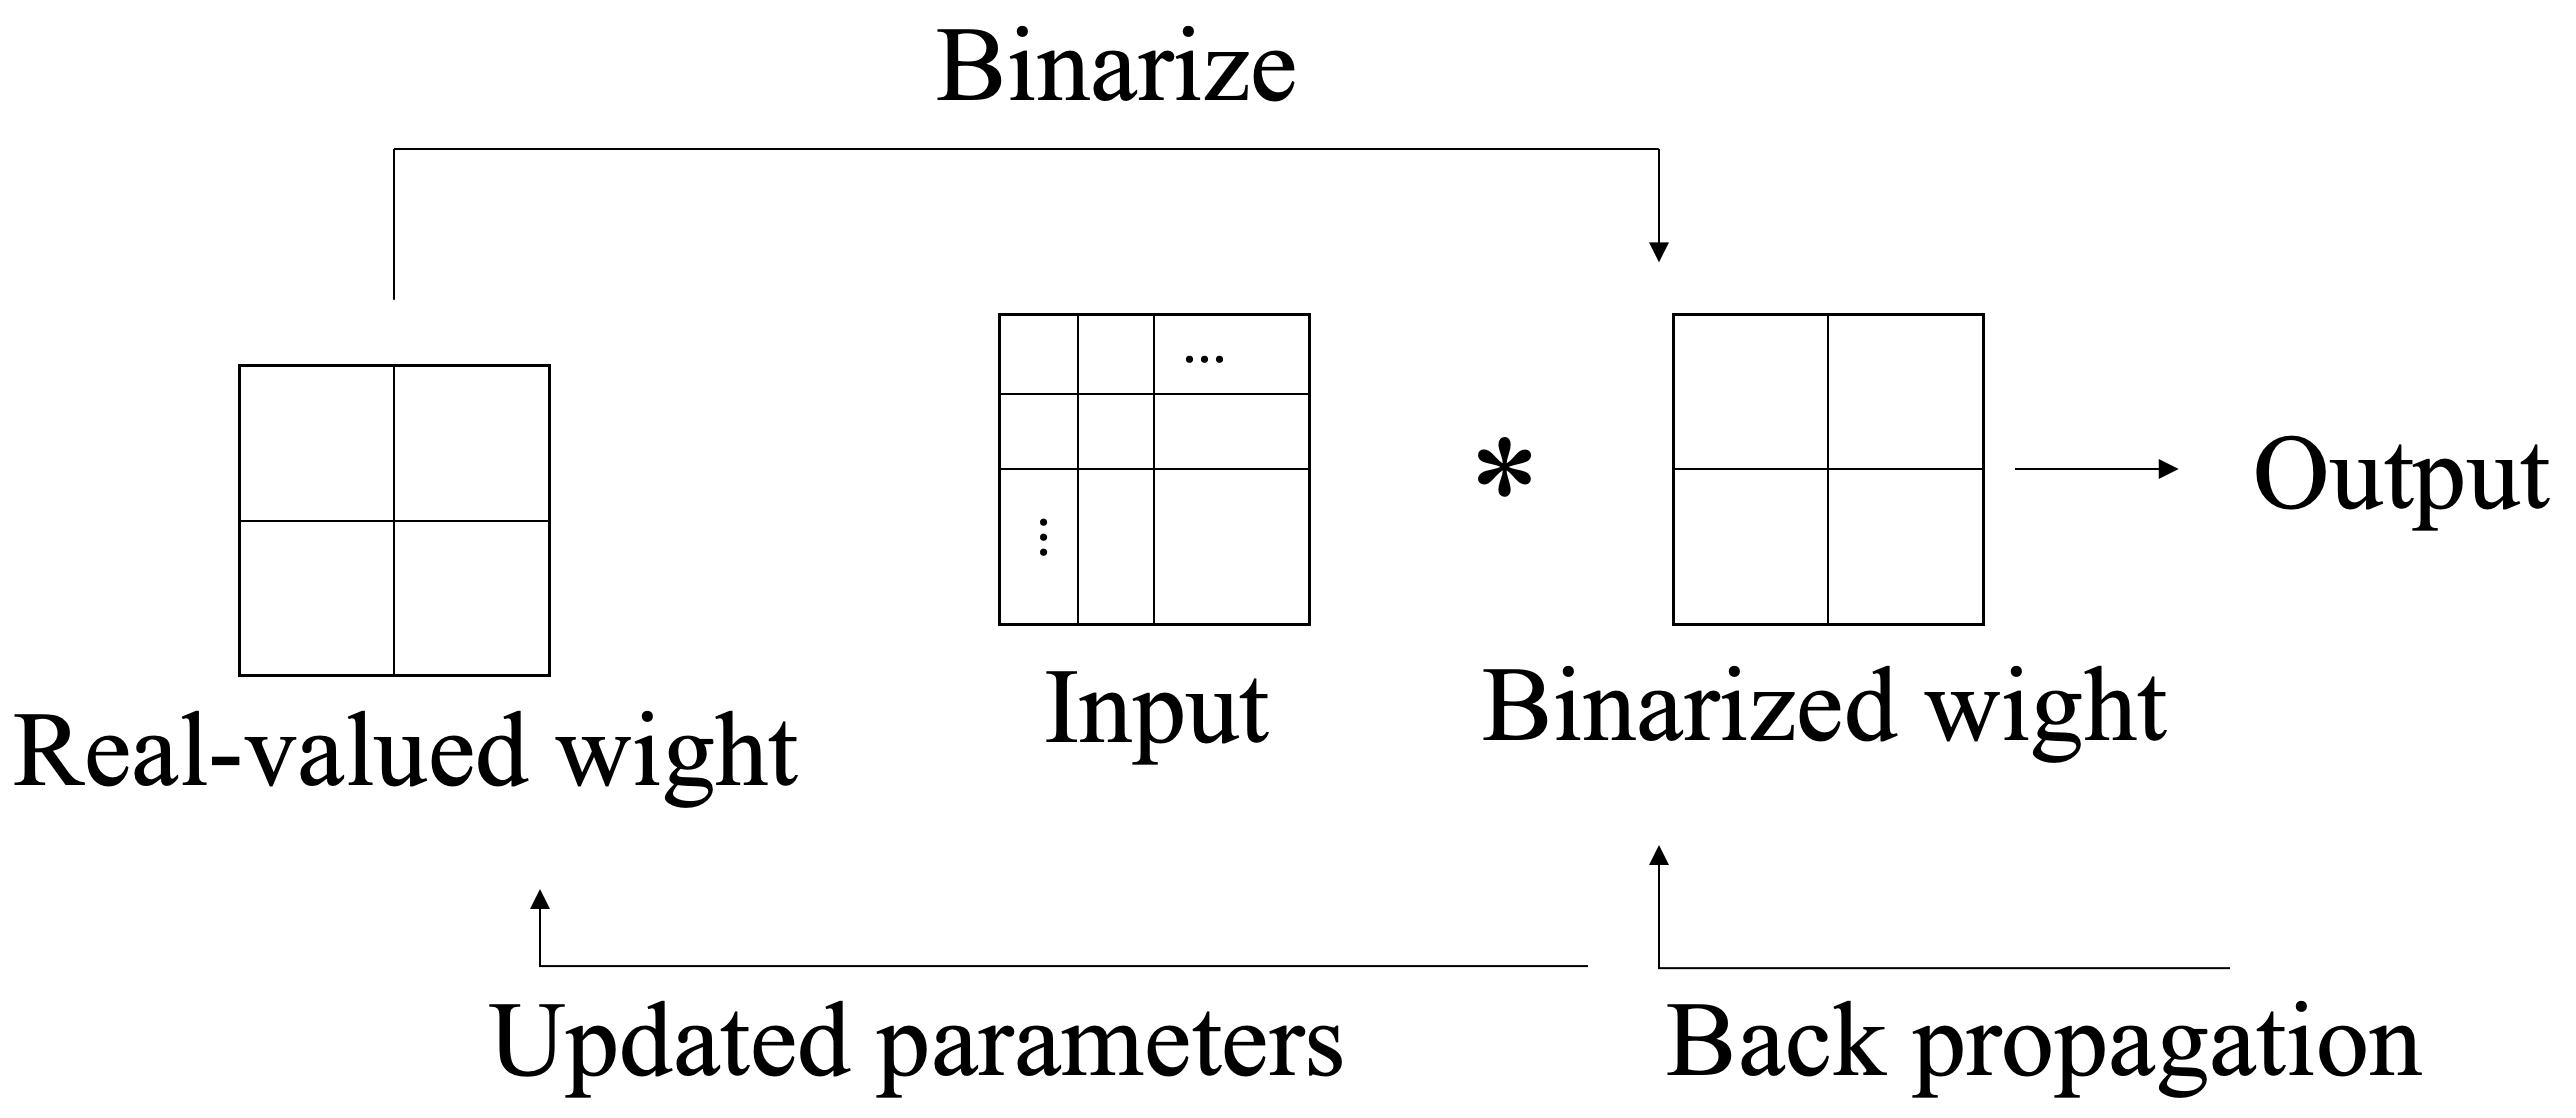
\includegraphics[scale = 0.25]{./chapter2/binarize.png}
    \caption{BinaryConnectにおけるパラメータ更新の流れ}
    \label{fig_binarize}
  \end{center}
\end{figure}